\begin{thm}{075}{\hosi ?}{}
 $\angle\mr{A}$の二等分線上に点Bを決め、線分ABを弦とする任意の円を描く。このとき、AP$+$AQの長さは円の大きさによらず一定となることを示せ。
 \begin{center}
  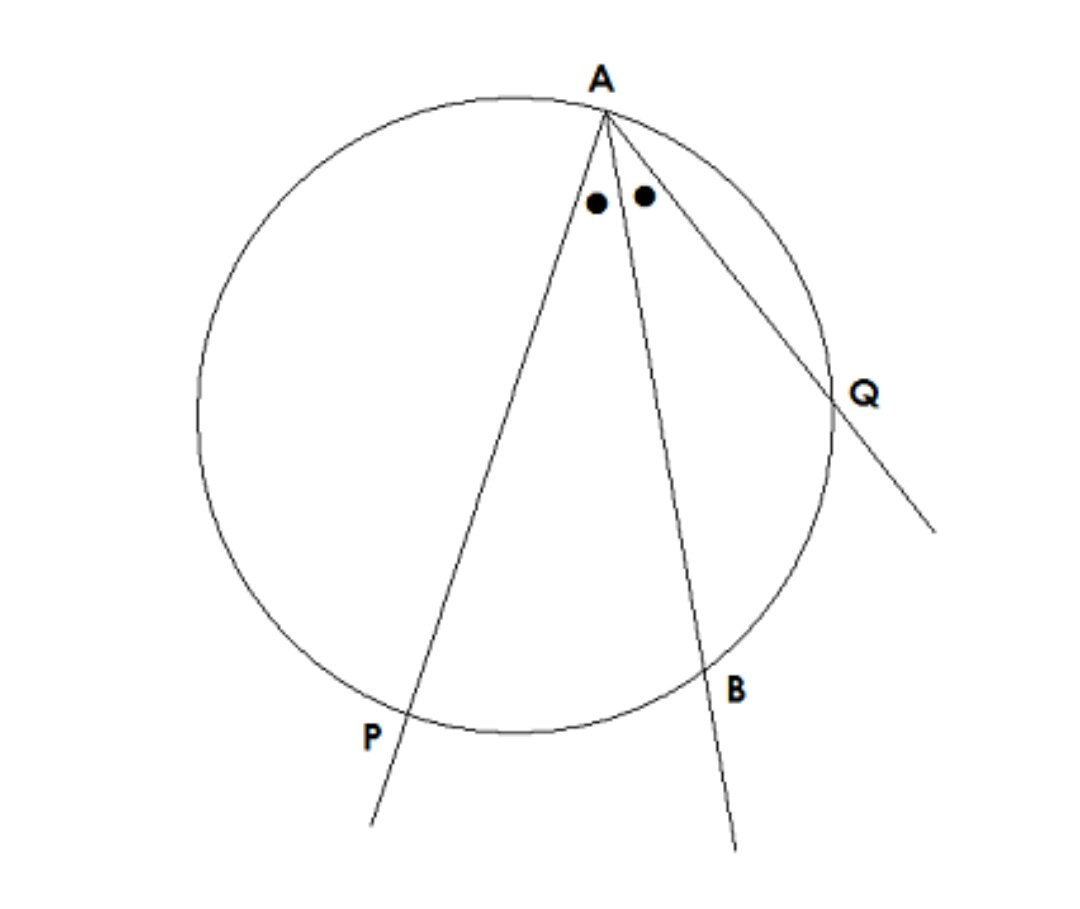
\includegraphics[bb=0 0 1080 909,width=0.7\linewidth]{../problems/Q_075/Q_075.jpg}
 \end{center}
\end{thm}

座標平面上で点Aを原点にとり、$a>0$なる定数$a$をおき、座標平面上の2直線$y=ax$と$y=-ax$をとる。ただし双方とも$x\ge 0$の範囲内のみ考える。すると$x$軸 ($x\ge 0$の部分) は$\angle\mr{A}$の2等分線になるから、この上に点Bを決める。ここでB$(2,0)$として一般性を失わない。線分ABを弦とするような任意の円は、$(x-1)^2+(y-t)^2=1+t^2$によってあらわされる。このとき、この円と$y=\pm ax$との$x>0$における交点がそれぞれP, Qとなるから、AP$+$AQが$t$によらないことを示せばよい。なお、$t$は点P, Qが存在する範囲内で動くものとする。
\begin{figure}[H]
 \centering
 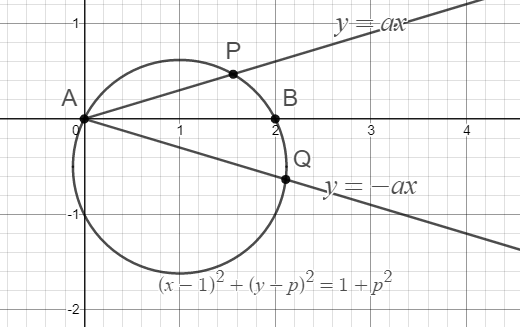
\includegraphics[width=0.7\linewidth]{../problems/Q_075/A_075.png}
\end{figure}

点P, Qの座標をそれぞれP$(p, ap)$, Q$(q, -aq)$とおく。ここで$p, q>0$。すると、
\[ \mr{AP}+\mr{AQ}=\sqrt{p^2+(ap)^2}+\sqrt{q^2+(-aq)^2}=(p+q)\sqrt{1+a^2} \]
である。直線$y=\pm ax$と円$(x-1)^2+(y-t)^2=1+t^2$の交点のうち原点でないものの$x$座標は、
\[ (x-1)^2+(\pm ax-t)^2=1+t^2 \]
を$x\neq 0$のもとで解いて、$x=\dfrac{2(1\pm at)}{1+a^2}$。したがって
\[ \mr{AP}+\mr{AQ}=(p+q)\sqrt{1+a^2}=\frac{2}{\sqrt{1+a^2}} \]
となって$t$によらないから、題意は示された。
